\documentclass[12pt]{article}

\usepackage{sbc-template}

\usepackage{graphicx,url}
\usepackage{tikz}
%\usepackage[brazil]{babel}   
\usepackage[utf8]{inputenc}
\usepackage{xcolor,listings}

\pagenumbering{alph}
\def\checkmark{\tikz\fill[scale=0.4](0,.35) -- (.25,0) -- (1,.7) -- (.25,.15) -- cycle;}
\sloppy

\title{Clear Exception Message Pattern}

\author{Eduardo Delgado Coloma Bier\inst{1}, Fernanda de Camargo Magano\inst{1}, \\ Fernando Freire Scattone\inst{1},
  Florence Alyssa Sakuma Shibata\inst{1}, Tallys Gustavo Martins\inst{1} }


\address{Instituto de Matemática de Estatística -- Universidade de São Paulo
  (USP)\\
  -- SP -- Brazil
  \email{\{eduardo.bier,fernanda.magano,fernando.scattone,florence.shibata\}@usp.br}
  \email{tallys@ime.br}
}

\pagenumbering{roman}

\begin{document} 

\maketitle

\begin{abstract}

Writing clear exception messages is useful for solving problems in the code faster, because the source of the issues are stated in a clear manner. Therefore, using a pattern for the exception messages brings consistency to the code and allows reuse inside of the same application or among different ones, since dealing with exceptions is an important part of every application. The current paper shows the ``Clear Exception Message Pattern''     developed by the authors, exposing the strengths and weaknesses, as well as known usages and the pattern format \cite{smith:99}, \cite{bernardo2008importancia}. 
  
\end{abstract}


\section{Introduction}

When developing a system, quality code is desirable to solve the proposed problems and meet the requirements. However, as the system becomes more complex, it is harder to isolate errors and bugs and fix them. The ability to detect, diagnose and handle these errors is essential to the maintenance and support of the final product. For such, mechanisms like log to detect errors at the moment they occur and obtain sufficient information about them, as well as  organized documentation of exceptions help developers to quickly and punctually fix them.

If the errors are handle incorrectly, they can reduce the usability of the system. For example, when errors are not handled and appear to the user of the application, they can confuse them and build a bad image of the system, that can be known as unreliable. If the message given in the exception isn't clear, the programmers will need more time to find and fix the problem and this delay can cost to the user of the system, like a company.

Even though there is a large variety of languages for application development, there is no standard documentation for handling exceptions or errors. Each developer is responsible for the task to generate some sort of mechanism for capturing and handling these cases. Aiming to simplify and fix bugs more easily the proposed Clear Exception Message Pattern seeks a standard to write messages in exceptions that are not too long but, at the same time, is sufficiently expressive  to understand what is the problem and where it occur.

This pattern can be used in projects of different domains, since catching exceptions is fundamental in every application developed in real world scenarios. It brings consistency and consequently allows the reuse of code.



%Maintaining a system is an important part of the software production and development  process. If developers have  mechanisms to detect errors the moment they occur and obtain sufficient information about them, they can find and fix bugs more easily. 
%If the given error message is incomplete or have inappropriate information it is difficult to maintain the application. It is important to find a meaningful and concise message  

\section{Pattern}
\begin{flushleft}
\textbf{Name:} Clear Exception Message Pattern\newline

\textbf{Type:}  Clarity \newline

\textbf{Intent:} Write exception messages that are specific to the domain of the application and easier to understand.\newline

\textbf{Motivation:}
When writing applications it is necessary to catch and treat exceptions that may arise. Since the messages should help the programmer better understand where the errors have occurred and how to fix them, it is important to have expressive messages when throwing an exception. 
Also, the developers of the programs maybe don't have all the technical expertise to understand all the exceptions from the native language, so it is useful to have exceptions that can indicate where the error occurred , what might be and maybe imply a common error in some cases.\newline

\textbf{Also Known As:} Error Message Pattern, Formatted Message Pattern\newline

\textbf{Pattern format description:}

\begin{figure}[!htb]
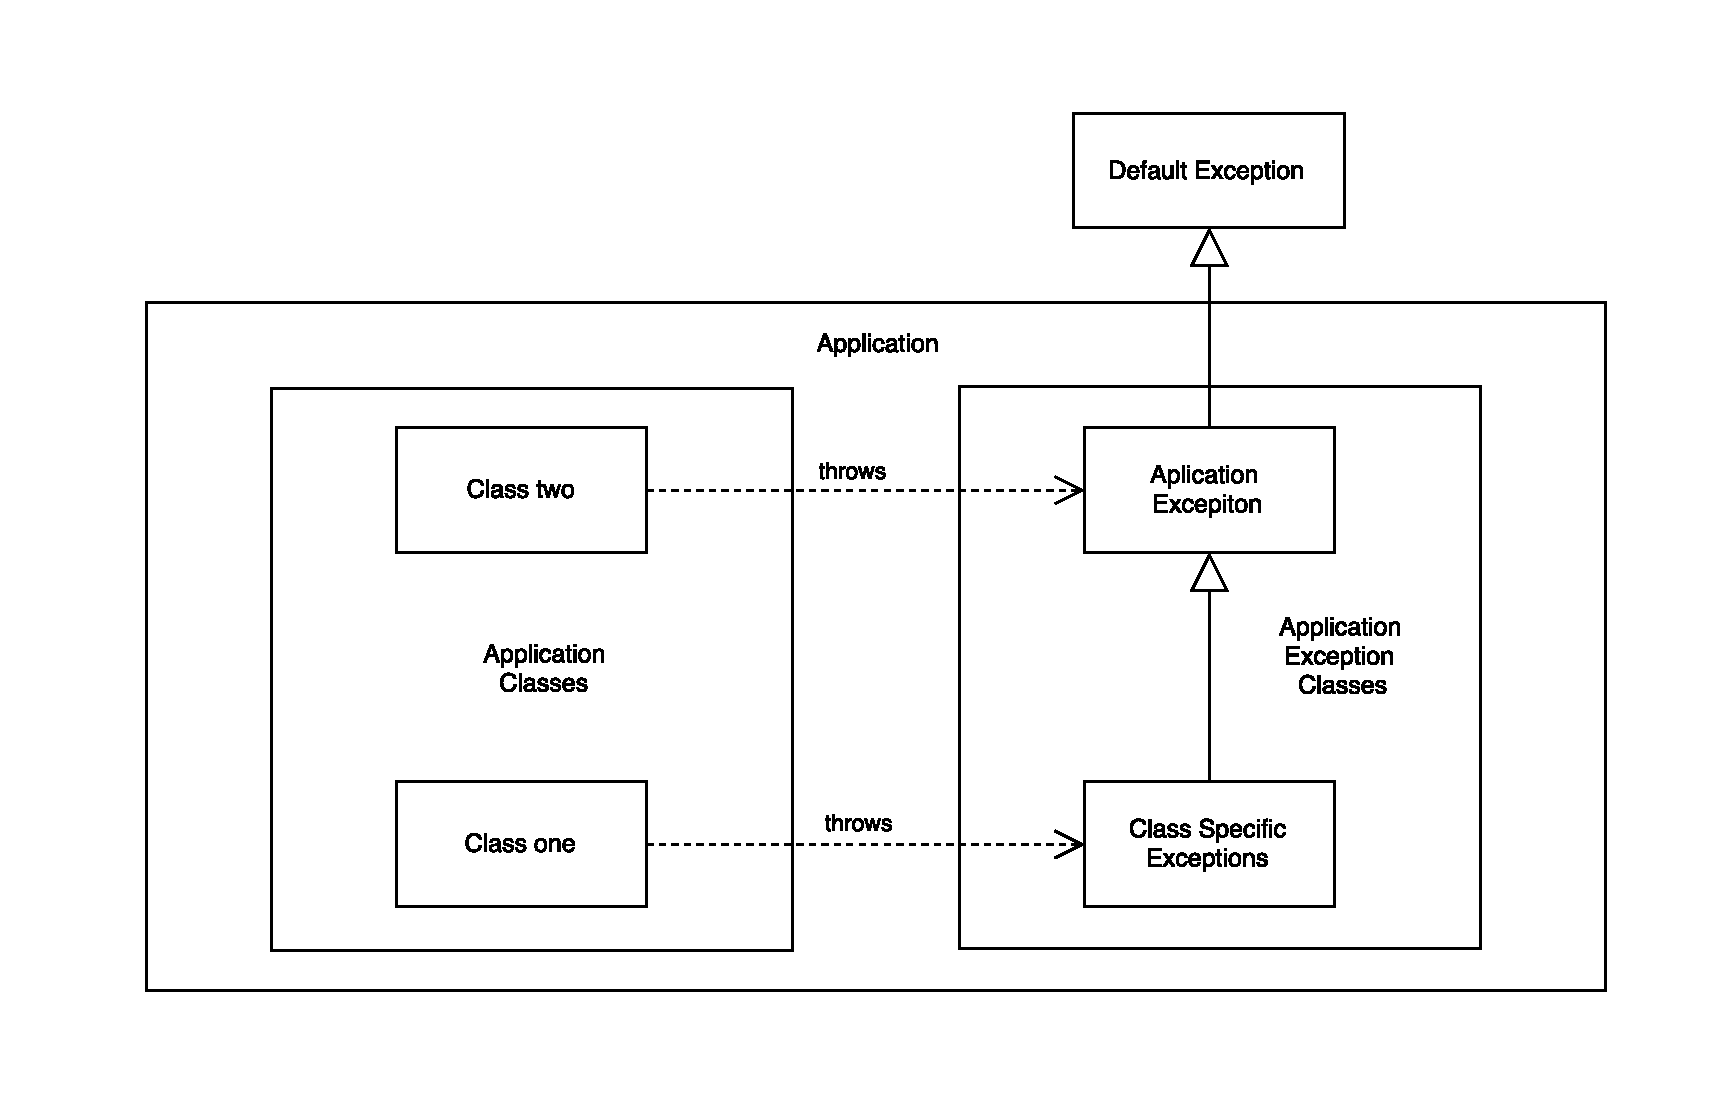
\includegraphics[width=\textwidth]{diagrama.pdf}
\caption{UML diagram of Clear Exception Message Pattern}
\label{UML-diagram}
\end{figure}

In the figure \ref{UML-diagram} is possible to see two application classes. In order to implement the Clear Exception Message Pattern is necessary to create, at least, an Application Exception Class, which will treat exceptions that may appear on most classes of the application. If needed, a specific Class of the application may have its own Class Specific Exception Class, that will inherit from the Application Exception Class all common exception treatments. 

\newpage
The Clear Exception Message Pattern deals with some kinds of exception handling messages:
 \begin{enumerate}
 \item Exception with files
 \item Exception with connection status
 \item Incompatible variable types 
  \end{enumerate} 
 
The first one treats common problems with files, like: not found, wrong permissions -- try to write in a file opened for reading. The second deals with connection issues. The pattern gives the example of failure to open TCP connection, but other possible issues are timeout, connection forbidden, among others. The last item refers to problems with conversion of types -- if the program sums numbers but among the variables are strings, for example.

A key point when rescuing errors that deserve attention is how generic the handled exception is. Catch the most specific exception as possible is important and is the best approach to be taken since generic errors are not clear and turn more difficult to encounter the error. So one of the goals of the current pattern is writing messages that catch specific exceptions. 
 
One exception has some information associated with it. Among them are the error type, the cause, the trace and they help to understand the exception itself. Then, the pattern messages will contain information about the type of the exception, a brief description and, when appropriated, some information about the trace like the line number when it occurred.


\textbf{Antagonic Forces:} While writing or using a program, the developer may do a wrong assignment type or try to open a file that does not exist or connect with an on-line address that is not available. These are not always errors on the code itself, but circumstances of the environment on which the code is being executed.If these errors occurred during production, the developer , when running the code, maybe will come against a difficult to interpret exception which may not give a friendly suggestion on where this error occurred. This happens, usually, because the language developers only write exceptions for very broad cases that cover various specif cases which the application developer may find difficult to find in they're own code, which may happen often in large scale projects.  \newline

\textbf{Strengths:} 

Among the strengths of this pattern it is possible to cite:
\begin{enumerate}
\item The messages will follow a pattern and will be similar to each other

\item It is consistent with previous messages used in other parts of the code.  

\item It provides succinct information of the error increasing the quality and readability of the code

\item It is clearer to understand how the codes works for other programmers that didn’t program the application

\item It helps the maintenance of the application and it's lifecycle management

\item  Informing specific error message allows robust framework implementation and program flow monitoring

%\textbf{[CASO NOSSO CÓDIGO TENHA TEMPLATE (algum lugar que centralize o tratamento de erros) - CASO NÃO TENHA, RETIRAR ESTE ITEM!]}
\item The improvement of exception handling later in the development process can be done easily in a single spot

\end{enumerate}



\textbf{Weaknesses:}

\begin{enumerate}
\item The amount of labor dedicated to finding possible exceptions that may occur might be too much to handle , depending on the team working the code, time constrains, and scale of the project.

\item There is a possibility of re-throw exceptions cases (chaining exceptions) causing loss of efficiency
\end{enumerate}%\textbf{Fernando}\newline 


\textbf{Consequences:}

\begin{enumerate}
%
\item Time and energy in finding errors will be reduced
\item By implementing specific exceptions for all cases the modularization of the software is improved
\item The pattern forces the developer to think about the exceptions of each Class, which may help them understand the project better and see if the requirements are being delivered
\end{enumerate}
%\textbf{Tallys}


\textbf{Known usages:}
Some prestigious languages such as Ruby and Python, already come with very detailed exception by default\newline
%\textbf{Eduardo}

\textbf{Recommended usage:}

\begin{enumerate}
\item Large projects where new people are joining and the production environment could be made a little bit friendlier by helping new programmers find their errors
\item Medium projects where the team is always changing and new members are not very familiar with the language they are using
\end{enumerate} 
%\textbf{Tallys}

\textbf{Discouraged usage:}
This pattern should not be used when:
\begin{enumerate}
\item The project is too small - The overhead to implement the pattern may not be worth the energy spending implementing.
\item The people who developed the software from the start are the same ones as in production - In this case, they are very familiar with the code and maybe they don't need this pattern in order to know where the exception appear
\end{enumerate}


\textbf{Code examples:}
The code examples -- shown in the appendix -- are written in two languages Ruby and Java. They were chosen for the example because Ruby is dynamic, while Java is a compiled language. So this comparison illustrates that it is possible to use the developed pattern in different types of programming languages.

% \lstinputlisting[language=Ruby]{codd.rb}

 %\begin{lstlisting}[
 %   label=listing:RubyTest,
  %  float=h,
%    caption=clear\_exceptions.rb,%
%    firstnumber=1,
  %  language=Ruby,
   % basicstyle=\ttfamily,
  %  keywordstyle=\color{red},
   % stringstyle=\color{blue},]

%#####CONNECTION#####

%#Wrong URL
%require 'open-uri'

%remote_base_url = "http://nonsense/"

%begin
  % rpage = open("#{remote_base_url}/")
%rescue SocketError=>e
  % puts "#{ e.class.name }: #{ e.message }"
%else
  % data = rpage.read
%end

% if data
  % File.open("url.html", "w"){|f| f.write(rdata) }
% end


%#####FILES#####

%#Wrong permission in file
%begin
%	File.open("/etc/hosts") {|f| f << "example"}
%rescue IOError => e
%	puts "#{ e.class.name }: #{ e.message } - #{ e.backtrace[3]}"
%end

%#File does not exist
%begin
%	File.open("does/not/exist")
%rescue Errno::ENOENT => e
%	puts "#{ e.class.name }: #{ e.message } - #{ e.backtrace[1]}"
%end

%#####DATA TYPE#####

%#Wrong type of data given by the user
%number = false
%while !number
  % puts "Write a number>>"
  % begin
  %   num = Kernel.gets.match(/\d+/)[0]
 %  rescue NoMethodError => e
 %    puts "#{ e.class.name }: #{ e.message }"
%     puts "\tWrite a number this type\n"
%   else  
%     puts "#{num} + 1 is: #{num.to_i+1}"
 %    number = true
 %  end  
%end

%\end{lstlisting}

 \end{flushleft}
 

\section{Conclusion}

The developed pattern treats specific exception handling messages, like file not found, connection issues, since the more specific is the exception caught, the clearer is the source of the problem. The readability of the messages, the possibility of code reuse and the facility in maintaining the system are the main goals of this pattern.

\bibliographystyle{sbc}
\bibliography{sbc-template}
\newpage


\lstinputlisting[language=Ruby, caption=clear\_exceptions.rb]{codd.rb}
\lstinputlisting[language=Java, caption=Exceptions.java]{Exceptions.java}
\end{document}
